

\begin{document}
	\maketitle
	\section*{سوال ‍۱‍  : }
	
	برای این که متوجه شویم که چه اتفاقی بر اثر این خطا رخ می دهد یک دستور 
	\lr{add}
	را بر روی این پردازنده انجام می دهیم  . به این صورت که ابتدا در رجیستر 
	\lr{R31}
	مقدار صفر را قرار و مقدار یک را داخل رجیستر 
	\lr{R30}
	قرار می دهیم و بعد دستور 
	\lr{add R30 , R31 , R31}
	 را اجرا می کنیم و انتظار داریم که در 
	 \lr{R30}
	 مقدار صفر ذخیره شده باشد ولی چون مقدار 
	 \lr{Write Register }
	 به خاطر خطا برابر با یک می باشد بنابراین نتیجه در رجیستر 
	 \lr{R31}
	 نوشته می شود و مقدار موجود در رجیستر 
	 \lr{R30}
	 همان یک باقی می ماند . همان طور که می بینیم در صورتی که در دستور خود بخواهیم بر نتیجه بر روی رجیستر با اندیس زوج ذخیره کنیم به خاطر این خطا مقدار نتیجه در رجیستر فرد نوشته می شود . بنابراین ما باید برنامه را طوری تغییر دهیم که فقط از رجیستر ها با اندیس زوج استفاده کند . 
	 \\
	 با این خطا همواره مقدار حاصل از دستورات 
	 \lr{branch}
	  نتیجه واکشی دستورات اشتباه می باشد که با توجه به این موضوع دیگر نمی توانیم هیچ دستور
	  \lr{branch}
	  ای را به صورت درست انجام دهیم پس پردازنده با این خطا غیر قابل استفاده است . 
	  \hrule
	  \section*{سوال۲  : }
	  همان طور که میدانیم دستور
	  \lr{LW}
	  نسبت به سایر دستورات زمانی بیشتری نیاز دارد  . 
	  \\
	\textbf{  با توجه به این که در صورت سوال قید نشده که تاخیر کدام بلوک را ۱۰ درصد کاهش می دهیم بنابراین 
	  \lr{SpeedUp}
	   را برای دستور گفته  شده به ازای کاهش تاخیر تمام بلوک ها به دست می آوریم : }
   \\
 ابتدا باید مشخص کنیم که برای این دستور از کدام بلوک های موجود در مسیرداده باید عبور کنیم  : 
   
   
   \begin{flushright}
 	\item  \lr{I-Mem}
 \item	 \lr{Regs}
 \item 	\lr{Mux} : برای انتخاب کردن ورودی 
 \item	 \lr{ALU}
 \item		 \lr{D-Mem}
 \item 		 \lr{Mux} : 
 برای انتخاب داده ای که باید در رجیستر نوشته شود
   \end{flushright}

با توجه به بالا مقدار زمان برای دستور مورد نظر قبل از کاهش به صورت زیر است  : 
\begin{center}
	$LW _{Time} = 200ps + 90ps + 20ps + 90ps + 250ps + 20ps = 670ps$
\end{center}

\subsection*{\lr{I-Mem}} 
حال ۱۰ درصد از تاخیر این بلوک کم می کنیم که برابر می شود با  
\textcolor{red}{\lr{$Delay_{IMem} = 180$}}
پس مقدار تاخیر برای دستور مورد نظر به صورت زیر می باشد  : 
 \begin{center}
 	$LW _{Time} = 180ps + 90ps + 20ps + 90ps + 250ps + 20ps = 650ps$
 \end{center}
بنابراین 
\lr{SpeedUp}
به صورت زیر می باشد  : 
\begin{center}

	$ = \frac{670}{650} = 1/0307 $	\lr{SpeedUp}
\end{center}

\subsection*{\lr{Add}}
با توجه به این که این واحد در مسیر این دستور قرار ندارد بنابراین کم کردن تاخیر این واحد  هیچ تاثیری در سرعت این دستور ندارد بنابراین در این حالت 
\lr{SpeedUp}
ای وجود ندارد . 
\subsection*{\lr{Mux}}
حال ۱۰ درصد از تاخیر این بلوک کم می کنیم که برابر می شود با  
\textcolor{red}{\lr{$Delay_{Mux} = 18$}}
پس مقدار تاخیر برای دستور مورد نظر به صورت زیر می باشد  :
 \begin{center}
	$LW _{Time} = 200ps + 90ps + 18ps + 90ps + 250ps + 18ps = 666ps$
\end{center}
بنابراین 
\lr{SpeedUp}
به صورت زیر می باشد  : 
\begin{center}
	
	$ = \frac{670}{666} = 1/0060 $	\lr{SpeedUp}
\end{center}
\subsection*{\lr{ALU}}
حال ۱۰ درصد از تاخیر این بلوک کم می کنیم که برابر می شود با  
\textcolor{red}{\lr{$Delay_{ALU} = 81$}}
پس مقدار تاخیر برای دستور مورد نظر به صورت زیر می باشد  :
\begin{center}
	$LW _{Time} = 200ps + 90ps + 20ps + 81ps + 250ps + 20ps = 661ps$
\end{center}
بنابراین 
\lr{SpeedUp}
به صورت زیر می باشد  : 
\begin{center}
	
	$ = \frac{670}{661} = 1/0136 $	\lr{SpeedUp}
\end{center}
\subsection*{\lr{Regs}}
چون زمان این بلاک به اندازه 
\lr{ALU}
می باشد بنابراین مقدار 
\lr{SpeedUp}
آن هم یکسان است و برابر است با 
\textcolor{blue}{1/0136}

\subsection*{\lr{D-Mem}}
حال ۱۰ درصد از تاخیر این بلوک کم می کنیم که برابر می شود با  
\textcolor{red}{\lr{$Delay_{DMem} = 225$}}
پس مقدار تاخیر برای دستور مورد نظر به صورت زیر می باشد  :
\begin{center}
	$LW _{Time} = 200ps + 90ps + 20ps + 90ps + 225ps + 20ps = 645ps$
\end{center}
بنابراین 
\lr{SpeedUp}
به صورت زیر می باشد  : 
\begin{center}
	
	$ = \frac{670}{645} = 1/0387 $	\lr{SpeedUp}
\end{center}
\subsection*{\lr{Sign-Extend}}
با توجه به این که این واحد در مسیر این دستور قرار ندارد بنابراین کم کردن تاخیر این واحد  هیچ تاثیری در سرعت این دستور ندارد بنابراین در این حالت 
\lr{SpeedUp}
ای وجود ندارد . 
\subsection*{\lr{Shift Left 2}}
با توجه به این که این واحد در مسیر این دستور قرار ندارد بنابراین کم کردن تاخیر این واحد  هیچ تاثیری در سرعت این دستور ندارد بنابراین در این حالت 
\lr{SpeedUp}
ای وجود ندارد . 
\subsection*{\lr{ALU Ctrl}}
با توجه به این که این واحد در مسیر این دستور قرار ندارد بنابراین کم کردن تاخیر این واحد  هیچ تاثیری در سرعت این دستور ندارد بنابراین در این حالت 
\lr{SpeedUp}
ای وجود ندارد . 
\newline
\newline
با توجه به مطالب بالا می توان دریافت که
\lr{SpeedUp}
برای این دستور در بهترین حالت مقداری برابر با 
\textcolor{blue}{1/0387}
دارد . 
\hrule
\section*{سوال ۳ : }
\subsection*{\textcolor{red}{الف}}
برای این قسمت جدول به صورت زیر می باشد   : 
\begin{center}
	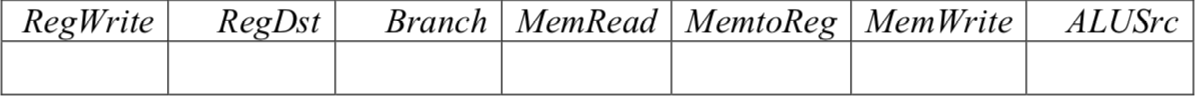
\includegraphics[width=1\textwidth]{beq}
\end{center}
\subsection*{\textcolor{red}{ب}}
برای این قسمت جدول به صورت زیر می باشد   :
\begin{center}
	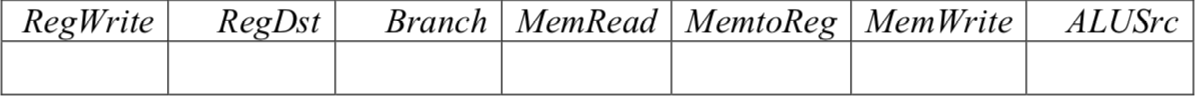
\includegraphics[width=1\textwidth]{beq}
\end{center}
\hrule
\section*{سوال ۴ : }
برای این کار باید یک سیگنال کنترلی به اسم 
\lr{\textcolor{red}{BNE}}
 به سیگنال های کنترلی خود اضافه کنیم در مرحله بعد باید یک گیت 
 \lr{AND}
 اضافه کنیم که ورودی های آن به شرح زیر می باشد  : 
 \begin{flushright}
 		
 	۱- سیگنال 
 	\lr{BNE}
 	\\
 	۲- خروجی 
 	\lr{ZERO}
 	مربوط به 
 	\lr{ALU}
 	را 
 	\lr{NOT}
 	می کنیم و به گیت 
 	\lr{AND}
 	می دهیم . (علت این کار در ادامه آمده است )
 \end{flushright}
برای این که بتوان دستور خواسته شده را پشتیبانی کرد باید به صورت زیر تغییرات را اعمال کنیم  : 
\begin{center}
	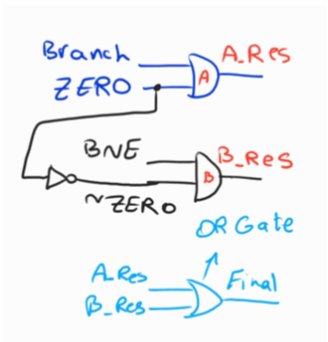
\includegraphics[width = 0.5\textwidth]{bne}
\end{center}
عللت استفاده از گیت 
\lr{OR}
این می باشد که پردازنده بتواند بعد از اعمال تغییرات هنوز هم از دستور 
\lr{BEQ}
پشتیبانی کند . 
\\
علت این که خروجی 
\lr{ZERO}
مربوط به 
\lr{ALU}
را 
\lr{NOT}
می کنیم این است که وقتی دو مقادیر موجود در دو رجیستر با یک دیگر برابر نیستند این خروجی مقدار صفر را به خود می گیرد که باعث می شود خروجی 
\lr{A-Res}
همواره صفر شود و در این صورت چون سیگنال کنترلی 
\lr{Branch}
را هم خودمان برابر صفر قرار دادیم پس خروجی 
\lr{B-Res}
نیز برابر با صفر می شود و بنابراین همواره خروجی 
\lr{Final}
برابر با صفر می شود پس همواره فقط مقدار 
\lr{PC}
را به 
\lr{PC + 4}
تغییر می دهیم که اشتباه است . به همین دلیل خروجی صفر 
\lr{ALU}
را 
\lr{NOT}
می کنیم . تا خروجی 
\lr{B-Res}
برابر با یک شود که باعث می شود خروجی 
\lr{Final}
یک شود و مالتی پلکسر مقدار 
\lr{PC}
را به 
\lr{PC + 4 + (imm<<2)}
تغییر می دهد و دستور 
\lr{BNE}
انجام می شود . 
\\ 
برای این که این دستور به درستی انجام شود مقادیر سیگنال های کنترلی به شرح زیر خواهد بود : 
\begin{center}
	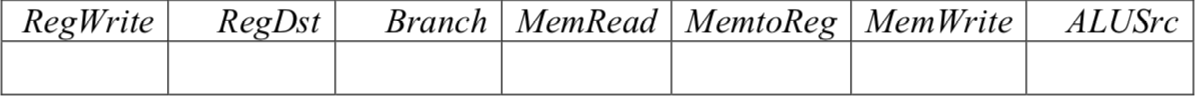
\includegraphics[width=1\textwidth]{beq}
\end{center}
\hrule
\section*{سوال ۵ : }
برای این منظور تنها کافی است مالتی پلکسری که ورودی 
\lr{MemtoReg}
دارد را تغییر داده و به جای آن از یک مالتی پلکسر ۳ به یک استفاده کنیم که در ورودی دوم خود مقدار 
\lr{PC}
را می گیرد . حال برای این که مقدار 
\lr{PC}
را داخل رجیستر 
\lr{rt}
قرار دهد باید سیگنال های کنترلی را به صورت زیر تغییر دهیم  : 
\begin{center}
	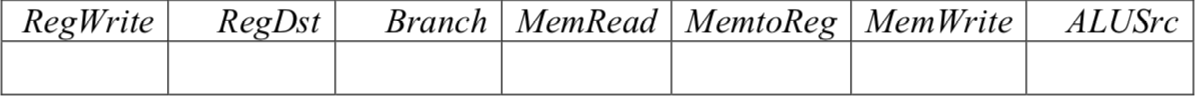
\includegraphics[width=1\textwidth]{beq}
\end{center}
\hrule
\section*{سوال ۶  : }
با توجه به این که دستور از نوع 
\lr{R-type}
می باشد بنابراین آدرس رجیستر مقصد در بیت های 
\lr{[15-11]}
می باشد پس 
\lr{\textcolor{red}{RegDst = 1}} . 
\\
چون نتیجه را می خواهیم در بانک ثبات ذخیره کنیم پس 
\lr{\textcolor{red}{RegWrite = 1}}
\\
چون این یک دستور 
\lr{Branch}
نیست پس 
\lr{\textcolor{red}{Branch = 0}}
\\
با توجه به این که دو مقدار خوانده شده را به عنوان ورودی به 
\lr{ALU}
می دهیم پس 
\lr{\textcolor{red}{ALUSrc = 0}}
\\
چون در این دستور نه از حافظه می خوانیم و نه بر روی حافظه می نویسیم پس  
\\ 
\lr{\textcolor{red}{MemRead = 0 , MemWrite = 0}}
\\
با توجه به این که مقدار خروجی از 
\lr{ALU}
را باید به بانک ثبات برگردانیم پس 
\lr{\textcolor{red}{MemtoReg = 0 }}
\\
چون دستور 
\lr{add}
داریم بنابراین 
\lr{\textcolor{red}{ALUOp  = 01 (ADD)}}
\\
همچنین چون دستور 
\lr{Branch }
نداریم مقدار 
\lr{PC}
را به 
\lr{PC+4}
تغییر می دهیم بنابراین 
\lr{\textcolor{red}{PC = 0x0016}}
\\
مقدار گذرگاه ها به شرح زیر می باشد  : 
\begin{center}
	\lr{\$ rt = \$ 10  = Instruction [20-16] = 01010}
	\\
	\lr{\$ rd  = \$20 = Instruction [15-11] = 10100}
	\\
	\lr{\$ rs = \$9 = Instruction [25-21] = 01001}
\end{center}
با توجه به مقادیر بالا داریم 
\begin{center}
	\lr{Read \  data1  = 1}
	\\
	\lr{Read \  data2 = 2}
	\\
	\lr{ALU \  Result  = 3}
\end{center}
\hrule
\end{document}